\chapter{Stworzony model zjawiska}

Niniejszy rozdział opisuje szczegółowo kolejne kroki oraz wykorzystane algorytmy niezbędne do uzyskania efektu końcowego.

%---------------------------------------------------------------------------

\section{Opracowanie danych topograficznych}
\subsection{Format .las}
Na początkowym etapie pracy otrzymano pliki w formacie .las - każdy z nich reprezentujący ukształtowanie terenu wybranego obszaru. 

Format .las został stworzony do przechowywania zbioru punktów w przestrzeni trójwymiarowej (ang. point cloud), otrzymanych przy pomocy metody Lidar, która polega na oświetlaniu wybranych punktów na powierzchni Ziemi laserem i zapisie jego odbicia przy pomocy sensorów. Dzięki tej metodzie powstają mapy o wysokiej rozdzielczości, stosowane w naukach o Ziemi (źródło: angielska wiki). 

Otrzymane pliki zawierały średnio około 11 milionów punktów, przy czym każdy z nich reprezentował powierzchnię ponad 2 km$^2$.

\begin{figure}[h]
	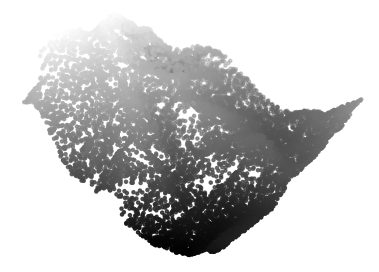
\includegraphics[width=8cm]{las_example}
	\centering
	\caption{Uproszczona wizualizacja zbioru punktów z pliku .las przy użyciu biblioteki matplotlib}
\end{figure}

\subsection{Wybór cech}
Jak wspomniano już wcześniej, do oszacowania ryzyka lawinowego konieczne jest posiadanie danych dotyczących cech terenu. Bazując na pracy pani Izabeli Woszczak, skupiono się na obliczeniu taki cech, jak:
\begin{itemize}
	\item forma terenu (skupiono się na żlebach);
	\item ekspozycja słoneczna;
	\item nachylenie powierzchni;
	\item piętro;
	\item wysokość.
\end{itemize}

\subsection{Triangulacja Delaunaya}
Sam zbiór punktów nie oferuje możliwości łatwego obliczania wyżej wymienionych cech, dlatego zastosowano uproszczenie powierzchni terenu przy pomocy triangulacji Delaunaya.

Jest to algorytm, który na podstawie zbioru punktów tworzy zbiór trójkątów, gdzie wierzchołki każdego trójkąta stanowią owe punkty. Własnością algorytmu jest, że maksymalizuje on najmniejsze z katów w powstałych trójkątach, unikając tzw. sliver triangles.

TE ZDJĘCIA POWINNY BYĆ DALEJ.

\begin{figure}[h]
	\centering
	\begin{minipage}{.5\textwidth}
		\centering
		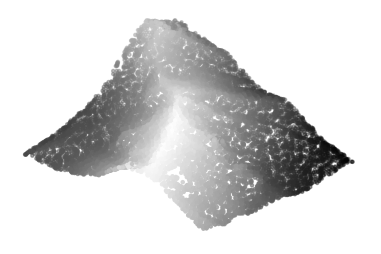
\includegraphics[width=.6\linewidth]{no_delaunay}
		\captionof{figure}{Obszar przedstawiony jako zbiór punktów}
		\label{fig:test1}
	\end{minipage}%
	\begin{minipage}{.5\textwidth}
		\centering
		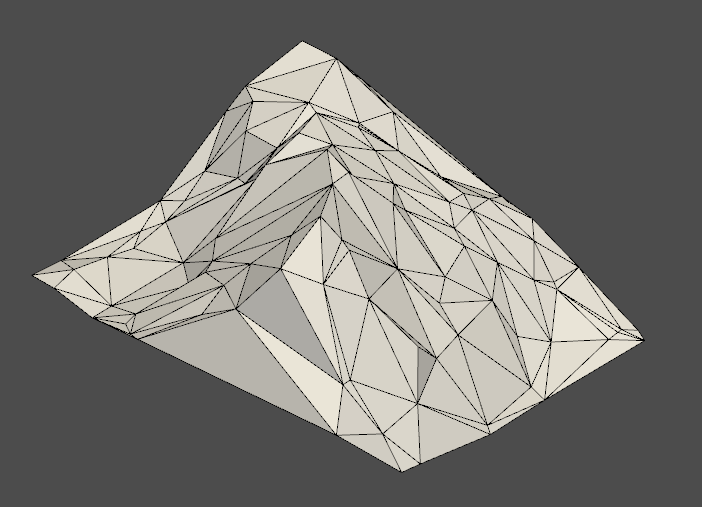
\includegraphics[width=.6\linewidth]{delaunay}
		\captionof{figure}{Ten samo obszar poddany triangulacji}
		\label{fig:test2}
	\end{minipage}
\end{figure}

Plik \LaTeX owy jest plikiem tekstowym, który oprócz tekstu zawiera polecenia formatujące ten tekst (analogicznie do języka HTML). Plik składa się z dwóch części:
\begin{enumerate}%[1)]
\item Preambuły -- określającej klasę dokumentu oraz zawierającej m.in. polecenia dołączającej dodatkowe pakiety;

\item Części głównej -- zawierającej zasadniczą treść dokumentu.
\end{enumerate}


\begin{lstlisting}
\documentclass[a4paper,12pt]{article}      % preambuła
\usepackage[polish]{babel}
\usepackage[utf8]{inputenc}
\usepackage[T1]{fontenc}
\usepackage{times}

\begin{document}                           % część główna

\section{Sztuczne życie}

% treść
% ąśężźćńłóĘŚĄŻŹĆŃÓŁ

\end{document}
\end{lstlisting}

Nie ma żadnych przeciwskazań do tworzenia dokumentów w~\LaTeX u w~języku polskim. Plik źródłowy jest zwykłym plikiem tekstowym i~do jego przygotowania można użyć dowolnego edytora tekstów, a~polskie znaki wprowadzać używając prawego klawisza \texttt{Alt}. Jeżeli po kompilacji dokumentu polskie znaki nie są wyświetlane poprawnie, to na 95\% źle określono sposób kodowania znaków (należy zmienić opcje wykorzystywanych pakietów).


%---------------------------------------------------------------------------

\section{Opracowanie danych pogodowych}
\label{sec:kompilacja}


Dane pogodowe potrzebne do symulacji zagrożenia 



%---------------------------------------------------------------------------

\section{Narzędzia}
\label{sec:narzedzia}


%---------------------------------------------------------------------------

\section{Przygotowanie dokumentu}
\label{sec:przygotowanieDokumentu}

Plik źródłowy \LaTeX a jest zwykłym plikiem tekstowym. Przygotowując plik
źródłowy warto wiedzieć o kilku szczegółach:

\begin{itemize}
\item
Poszczególne słowa oddzielamy spacjami, przy czym ilość spacji nie ma znaczenia.
Po kompilacji wielokrotne spacje i tak będą wyglądały jak pojedyncza spacja.
Aby uzyskać {\em twardą spację}, zamiast znaku spacji należy użyć znaku {\em
tyldy}.

\item
Znakiem końca akapitu jest pusta linia (ilość pusty linii nie ma znaczenia), a
nie znaki przejścia do nowej linii.

\item
\LaTeX~sam formatuje tekst. \textbf{Nie starajmy się go poprawiać}, chyba, że
naprawdę wiemy co robimy.
\end{itemize} 


